\section{Data storage and management system}

%%%%%%%%%%%%%%%%%%%%%%%%
\subsection{Data characteristics}
The characteristics of the raw \pdsp data are defined by the
properties of the TPC:
\begin{itemize}
\item the multiple wire planes, the fine wire pitch, and the resulting high channel count;
\item high digitization frequency (which is essential to ensure a precise position measurement along the drift direction); and
\item relatively slow drift velocity of electrons in LAr, which requires a readout window of the order of milliseconds  to collect
the ionization in the LAr volume stemming from the event of interest and overlapping cosmic rays.
\end{itemize}

%\noindent 
Triggered readouts of the detector (events), 
contain a large amount of raw data, impacting the bandwidth and
storage requirements.   The run plan, described in Section~\ref{sec:runplan},  determines the total number of events, and thus 
helps define the design requirements for the data storage and management system.

The \textit{\pdsp Data Scenarios} spreadsheet\,\cite{data_spreadsheet}  %(DUNE DocDB 1086)
describes a few possible running conditions. It includes estimates for their
resulting data volumes and rates, and interpretations of these estimates in terms of
network and disk bandwidth. The set of conditions labeled as \textit{Central} represents the most likely scenario
and is matched to the run plan.
Estimates are also provided for data taken out of the spills in order to measure the contributions from cosmic rays.
Table~\ref{tab:goldi} summarizes these estimates.

Based on the estimated event size quoted in Table~\ref{tab:goldi},  the anticipated total raw data volume to be 
taken during the planned SPS run is 3\,PB.



%%%%%%%%%%%%%%%%%%%%%%%%
\subsection{Raw data flow}
\label{sec:raw_concept}

\begin{cdrfigure}[Conceptual diagram of the flow of raw data in \pdsp]{raw_concept}{Conceptual diagram of the flow of raw data in \pdsp} 
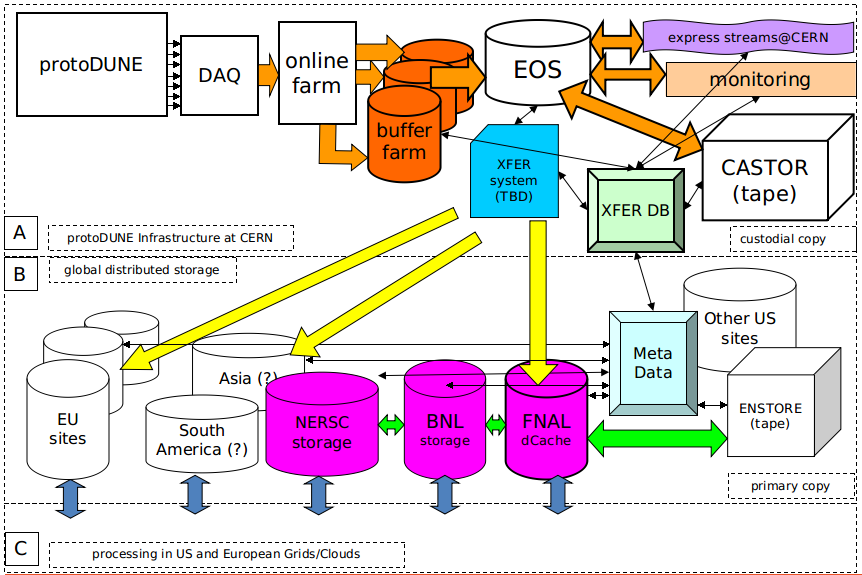
\includegraphics[width=\linewidth]{protoDUNE_raw_data_concept.png}
\end{cdrfigure}



A conceptual diagram of the raw data flow is presented in Figure~\ref{fig:raw_concept}. It shows the general logic
of the data flow and does not rely on assumptions of specific technical implementations. 
It also reflects the central role of CERN EOS in the raw data management scheme, which is motivated by the experience
and architecture of the LHC experiments.
\fixme{what's EOS?}

EOS serves as the staging area from which the data are committed to CASTOR (a hierarchical storage management system developed at CERN)
and from which data are transmitted to a number of endpoints including principal data centers such as Fermilab and others.
It is also used to provide input to QA and other express processing streams at CERN (Section~\ref{sec:prompt_processing}).


